\documentclass{article}\usepackage[]{graphicx}\usepackage[]{color}
%% maxwidth is the original width if it is less than linewidth
%% otherwise use linewidth (to make sure the graphics do not exceed the margin)
\makeatletter
\def\maxwidth{ %
  \ifdim\Gin@nat@width>\linewidth
    \linewidth
  \else
    \Gin@nat@width
  \fi
}
\makeatother

\definecolor{fgcolor}{rgb}{0.345, 0.345, 0.345}
\newcommand{\hlnum}[1]{\textcolor[rgb]{0.686,0.059,0.569}{#1}}%
\newcommand{\hlstr}[1]{\textcolor[rgb]{0.192,0.494,0.8}{#1}}%
\newcommand{\hlcom}[1]{\textcolor[rgb]{0.678,0.584,0.686}{\textit{#1}}}%
\newcommand{\hlopt}[1]{\textcolor[rgb]{0,0,0}{#1}}%
\newcommand{\hlstd}[1]{\textcolor[rgb]{0.345,0.345,0.345}{#1}}%
\newcommand{\hlkwa}[1]{\textcolor[rgb]{0.161,0.373,0.58}{\textbf{#1}}}%
\newcommand{\hlkwb}[1]{\textcolor[rgb]{0.69,0.353,0.396}{#1}}%
\newcommand{\hlkwc}[1]{\textcolor[rgb]{0.333,0.667,0.333}{#1}}%
\newcommand{\hlkwd}[1]{\textcolor[rgb]{0.737,0.353,0.396}{\textbf{#1}}}%

\usepackage{framed}
\makeatletter
\newenvironment{kframe}{%
 \def\at@end@of@kframe{}%
 \ifinner\ifhmode%
  \def\at@end@of@kframe{\end{minipage}}%
  \begin{minipage}{\columnwidth}%
 \fi\fi%
 \def\FrameCommand##1{\hskip\@totalleftmargin \hskip-\fboxsep
 \colorbox{shadecolor}{##1}\hskip-\fboxsep
     % There is no \\@totalrightmargin, so:
     \hskip-\linewidth \hskip-\@totalleftmargin \hskip\columnwidth}%
 \MakeFramed {\advance\hsize-\width
   \@totalleftmargin\z@ \linewidth\hsize
   \@setminipage}}%
 {\par\unskip\endMakeFramed%
 \at@end@of@kframe}
\makeatother

\definecolor{shadecolor}{rgb}{.97, .97, .97}
\definecolor{messagecolor}{rgb}{0, 0, 0}
\definecolor{warningcolor}{rgb}{1, 0, 1}
\definecolor{errorcolor}{rgb}{1, 0, 0}
\newenvironment{knitrout}{}{} % an empty environment to be redefined in TeX

\usepackage{alltt}
\usepackage{hyperref}
\hypersetup{colorlinks,% 
                 urlcolor=blue}
\author{Giusi Moffa \\[2ex] Statistical bioinformatics, University of Regensburg\\[4ex]}
\title{A \texttt{knitr} + \LaTeX~ dynamic report.\\[4ex]}
\date{27 May 2014 \\[4ex] Practical bioinformatics}
\IfFileExists{upquote.sty}{\usepackage{upquote}}{}

\begin{document}
\maketitle
\section*{p-values, one big topic for reproducible findings}
So let's look at how we can get a dynamic and reproducible report with `knitr`, for getting in the news.

\subsubsection*{Recording the $R$ session.}
It may be useful since different versions in general will not produce identical results.

\begin{kframe}
\begin{alltt}
\hlcom{# Print R session info}
\hlkwd{toLatex}\hlstd{(}\hlkwd{sessionInfo}\hlstd{())}
\end{alltt}
\end{kframe}\begin{itemize}\raggedright
  \item R version 3.0.3 (2014-03-06), \verb|x86_64-apple-darwin10.8.0|
  \item Locale: \verb|en_GB.UTF-8/en_GB.UTF-8/en_GB.UTF-8/C/en_GB.UTF-8/en_GB.UTF-8|
  \item Base packages: base, datasets, graphics, grDevices,
    methods, stats, utils
  \item Other packages: knitr~1.5
  \item Loaded via a namespace (and not attached): evaluate~0.5.5,
    formatR~0.10, stringr~0.6.2, tools~3.0.3
\end{itemize}



It is a good habit also to set your working directory and check whether you are in the right place.

\begin{knitrout}
\definecolor{shadecolor}{rgb}{0.969, 0.969, 0.969}\color{fgcolor}\begin{kframe}
\begin{alltt}
\hlkwd{setwd}\hlstd{(}\hlstr{"~/juicy/BioStatWork2012/mytex/journalClub/Reproducibility/repBioInfo"}\hlstd{)}
\hlkwd{getwd}\hlstd{()}  \hlcom{## obtain the working directory}
\end{alltt}
\begin{verbatim}
## [1] "/Users/giusimoffa/juicy/BioStatWork2012/mytex/journalClub/Reproducibility/repBioInfo"
\end{verbatim}
\end{kframe}
\end{knitrout}



\subsubsection*{One old trick for getting in the news}
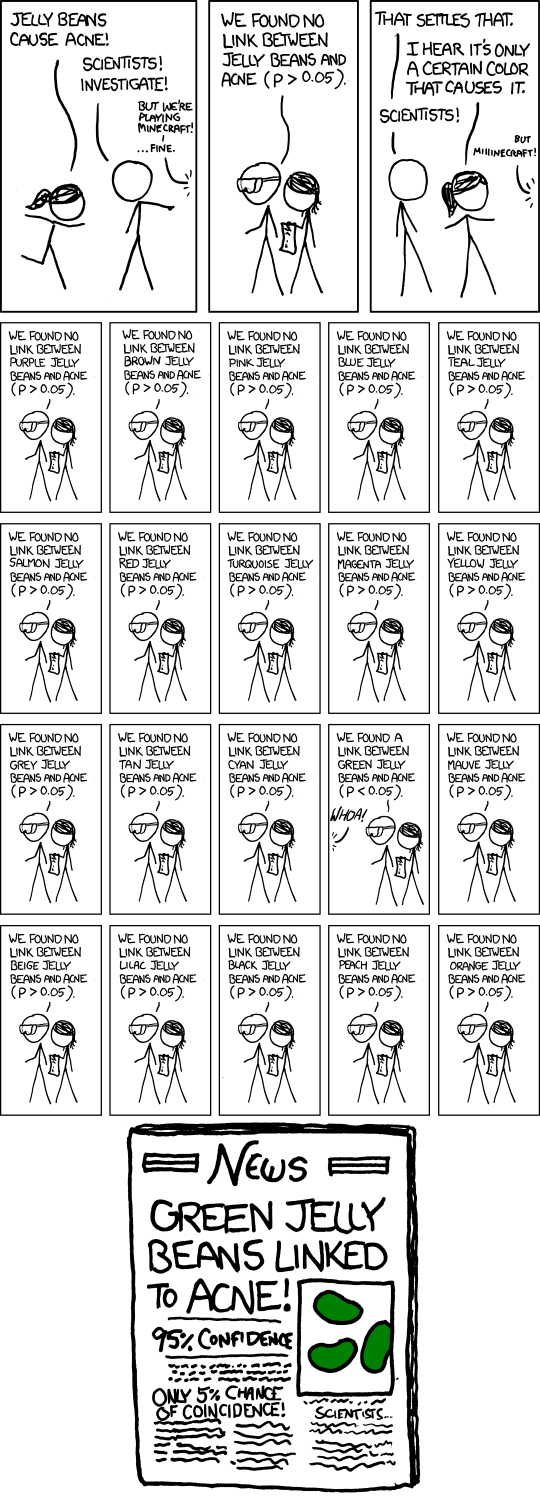
\includegraphics[width=.6\textwidth]{figure/significant.png}
%\clearpage

Under the null-hypothesis p-values are expected to be uniformly distributed between 0 and 1. So if we have hundreds of crazy hypotheses we can try a fishing expedition for significance by testing all of them. On average 5% will come up as significant.

\begin{knitrout}
\definecolor{shadecolor}{rgb}{0.969, 0.969, 0.969}\color{fgcolor}\begin{kframe}
\begin{alltt}
\hlkwd{set.seed}\hlstd{(}\hlnum{31}\hlstd{)}
\hlstd{nColors} \hlkwb{<-} \hlnum{200}
\hlstd{nObs} \hlkwb{<-} \hlnum{100}
\hlstd{jellyBeans} \hlkwb{<-} \hlkwd{matrix}\hlstd{(}\hlkwd{rnorm}\hlstd{(nObs} \hlopt{*} \hlstd{nColors),} \hlkwc{ncol} \hlstd{= nColors)}
\hlstd{fishing4News} \hlkwb{<-} \hlkwd{apply}\hlstd{(jellyBeans,} \hlnum{2}\hlstd{,} \hlkwa{function}\hlstd{(}\hlkwc{x}\hlstd{)} \hlkwd{t.test}\hlstd{(x)}\hlopt{$}\hlstd{p.value)}
\end{alltt}
\end{kframe}
\end{knitrout}


If we like simple numbers we can look at a table of summaries (here only for a small number of variables, for space constraints)
\begin{kframe}
\begin{alltt}
\hlkwd{library}\hlstd{(xtable)}
\hlkwd{xtable}\hlstd{(}\hlkwd{summary}\hlstd{(jellyBeans[,}\hlnum{1}\hlopt{:}\hlnum{4}\hlstd{]),}
       \hlkwc{caption}\hlstd{=}\hlstr{"Some variables' summaries"}\hlstd{)}
\end{alltt}
\end{kframe}% latex table generated in R 3.0.3 by xtable 1.7-3 package
% Wed May 28 14:39:02 2014
\begin{table}[ht]
\centering
\begin{tabular}{rllll}
  \hline
 &       V1 &       V2 &       V3 &       V4 \\ 
  \hline
1 & Min.   :-2.5408   & Min.   :-2.2187   & Min.   :-2.3257   & Min.   :-2.523   \\ 
  2 & 1st Qu.:-0.6512   & 1st Qu.:-0.6141   & 1st Qu.:-0.7047   & 1st Qu.:-0.425   \\ 
  3 & Median :-0.0442   & Median : 0.0846   & Median :-0.1013   & Median : 0.193   \\ 
  4 & Mean   :-0.0151   & Mean   : 0.0628   & Mean   :-0.0306   & Mean   : 0.113   \\ 
  5 & 3rd Qu.: 0.6460   & 3rd Qu.: 0.7606   & 3rd Qu.: 0.7086   & 3rd Qu.: 0.889   \\ 
  6 & Max.   : 2.3414   & Max.   : 2.2036   & Max.   : 2.6253   & Max.   : 2.159   \\ 
   \hline
\end{tabular}
\caption{Some variables' summaries} 
\end{table}



A graph might be more pleasant. The distribution can be visualised through the `hist` function and `density` function.
\begin{knitrout}
\definecolor{shadecolor}{rgb}{0.969, 0.969, 0.969}\color{fgcolor}\begin{kframe}
\begin{alltt}
\hlkwd{hist}\hlstd{(fishing4News,} \hlkwc{col}\hlstd{=}\hlnum{4}\hlstd{,} \hlkwc{breaks}\hlstd{=}\hlnum{20}\hlstd{,} \hlkwc{freq}\hlstd{=}\hlnum{FALSE}\hlstd{,}
     \hlkwc{main}\hlstd{=}\hlstr{"Distribution of p-values"}\hlstd{,} \hlkwc{xlab}\hlstd{=}\hlstr{"p-values"}\hlstd{)}
\hlkwd{lines}\hlstd{(}\hlkwd{density}\hlstd{(fishing4News),} \hlkwc{col}\hlstd{=}\hlnum{2}\hlstd{,} \hlkwc{lwd}\hlstd{=}\hlnum{2}\hlstd{)}
\end{alltt}
\end{kframe}
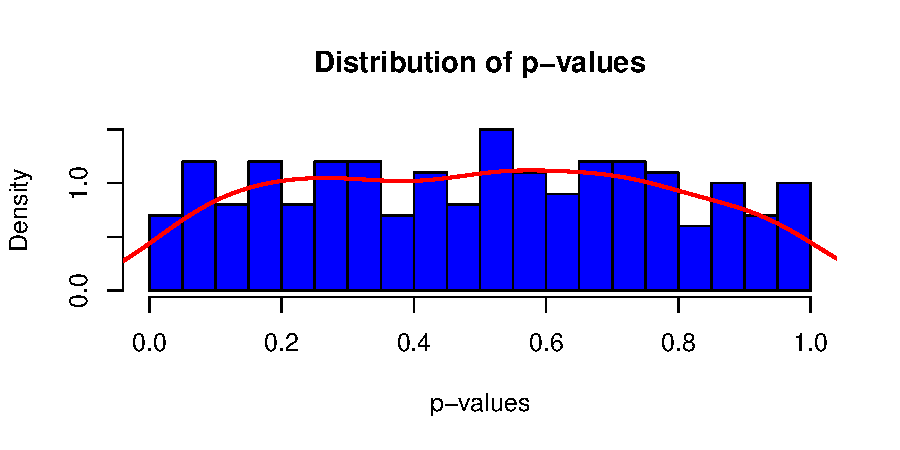
\includegraphics[width=\maxwidth]{figure/rFigFishing} 

\end{knitrout}


This way we get `r length(which(fishing4News<.05))` significant results. This problem is well known in genomics and adressed by a plethora of methods for multiple correction. Transparency however is not always necessarily guaranteed, especially in in fields such as social science, and the issue is still a very much debated hot topic. (E.g. \href{http://www.stat.columbia.edu/~gelman/research/unpublished/p_hacking.pdf}{The garden of forking paths: Why multiple comparisons can be a problem,
even when there is no "fishing expedition" or "$p$-hacking" and the research
hypothesis was posited ahead of time}). 
% Berger claims that the problem of multiple comparisons is ignored in epidemiology

\subsubsection*{Correction for multiple testing}
One way to account for multiple testing is by adopting the Benjamini-Hochberg correction. If we are "lucky" we can still get in the news after correcting for multiple testing, but we might need a rather larger number of crazy ideas.
\begin{knitrout}
\definecolor{shadecolor}{rgb}{0.969, 0.969, 0.969}\color{fgcolor}\begin{kframe}
\begin{alltt}
\hlkwd{set.seed}\hlstd{(}\hlnum{7}\hlstd{)}
\hlstd{nColors} \hlkwb{<-} \hlnum{10000}
\hlstd{nObs} \hlkwb{<-} \hlnum{20}
\hlstd{jellyBeans} \hlkwb{<-} \hlkwd{matrix}\hlstd{(}\hlkwd{rnorm}\hlstd{(nObs} \hlopt{*} \hlstd{nColors),} \hlkwc{ncol} \hlstd{= nColors)}
\hlstd{fishing4News} \hlkwb{<-} \hlkwd{apply}\hlstd{(jellyBeans,} \hlnum{2}\hlstd{,} \hlkwa{function}\hlstd{(}\hlkwc{x}\hlstd{)} \hlkwd{t.test}\hlstd{(x)}\hlopt{$}\hlstd{p.value)}
\hlstd{BHfishing} \hlkwb{<-} \hlkwd{p.adjust}\hlstd{(fishing4News,} \hlstr{"BH"}\hlstd{)}
\end{alltt}
\end{kframe}
\end{knitrout}


When testing for `r nColors` colours, and with a limited number (`r nObs` in this case) of observations we still get one significant result. However only `r length(which(BHfishing < .8))` are below .8.
\begin{knitrout}
\definecolor{shadecolor}{rgb}{0.969, 0.969, 0.969}\color{fgcolor}\begin{kframe}
\begin{alltt}
\hlkwd{min}\hlstd{(BHfishing)}
\end{alltt}
\begin{verbatim}
## [1] 0.01483
\end{verbatim}
\begin{alltt}
\hlkwd{sort}\hlstd{(BHfishing)[}\hlnum{1}\hlopt{:}\hlnum{5}\hlstd{]}
\end{alltt}
\begin{verbatim}
## [1] 0.01483 0.07893 0.83831 0.83831 0.83831
\end{verbatim}
\end{kframe}
\end{knitrout}


\begin{knitrout}
\definecolor{shadecolor}{rgb}{0.969, 0.969, 0.969}\color{fgcolor}\begin{kframe}
\begin{alltt}
\hlkwd{hist}\hlstd{(BHfishing,} \hlkwc{col}\hlstd{=}\hlnum{4}\hlstd{,} \hlkwc{breaks}\hlstd{=}\hlnum{20}\hlstd{,} \hlkwc{freq}\hlstd{=}\hlnum{FALSE}\hlstd{,}
     \hlkwc{main}\hlstd{=}\hlstr{"Distribution of adjusted p-values"}\hlstd{,}
     \hlkwc{xlab}\hlstd{=}\hlstr{"Benjamini-Hochberg adjusted p-values"}\hlstd{)}
\end{alltt}
\end{kframe}
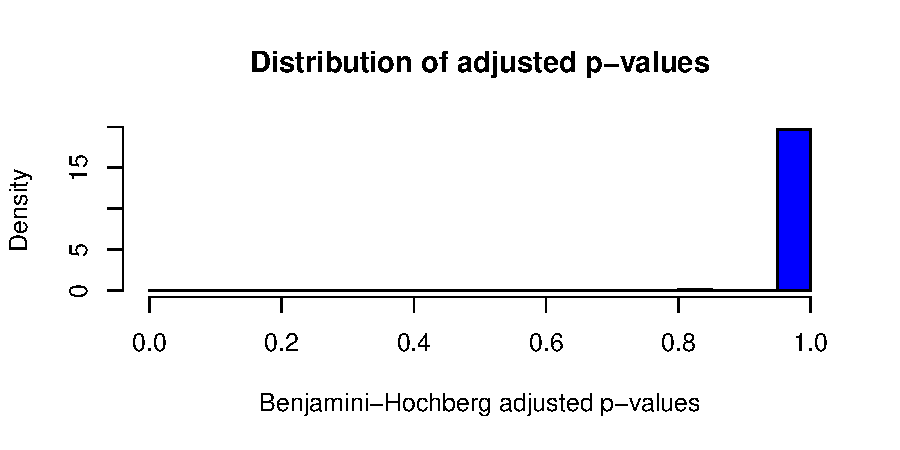
\includegraphics[width=\maxwidth]{figure/rFigBHfishing} 

\end{knitrout}


And if you really feel you need to, you can also save (and load) your entire workspace
\begin{knitrout}
\definecolor{shadecolor}{rgb}{0.969, 0.969, 0.969}\color{fgcolor}\begin{kframe}
\begin{alltt}
\hlkwd{save.image}\hlstd{(}\hlkwc{file} \hlstd{=} \hlstr{"fishing.RData"}\hlstd{)}
\hlkwd{load}\hlstd{(}\hlkwc{file} \hlstd{=} \hlstr{"fishing.RData"}\hlstd{)}
\end{alltt}
\end{kframe}
\end{knitrout}


\subsubsection*{Disclaimer}
This report is freely available for the benefit of **science**, so that our steps on the way to the news can be checked by anybody who wishes to do so.

\end{document}
